\documentclass[../improvements.tex]{subflies}

\begin{document}
  プロセッサが動的分岐予測機能を持つ場合, 
  分岐する時に無駄になるクロックサイクル数を減らすことができる.
  この節では, 今回の設計における動的分岐予測の実装方法と評価結果について述べる.

  \subsubsection{分岐予測の対象命令}
  分岐予測の対象命令を, 無条件分岐命令と条件付き分岐命令 
  (それぞれ表 \ref{table:isa} にある J形式と B形式の命令) とする.
  無条件分岐命令は必ず分岐し, 条件付き分岐命令よりも予測しやすいため, 
  分岐予測の対象に含めることにした.

  \subsubsection{分岐方向と分岐アドレスの予測方法}
  無条件分岐命令と条件付き分岐命令の予測しやすさに違いがあるため, 
  命令ごとに予測できるローカル予測器を採用した\cite{ca-quantitative-approach}.
  実装では, エントリー数が 32 の参照テーブル (図 \ref{fig:predictor-table}) を用意した.
  命令のアドレスの下位2ビットは常に \verb|00| であるため, 
  参照テーブルのエントリーは, 対象命令のアドレスの 6ビット目から 2ビット目までの値で指定する.
  そして, 1つのエントリーに $2\unit{\bit}$ の状態信号と $32\unit{\bit}$ の分岐先アドレスを保持する.
  状態信号の値と分岐方向の予測を表 \ref{table:predictor-state} に示す.

  \begin{figure}
    \resizebox{\columnwidth}{!}{
      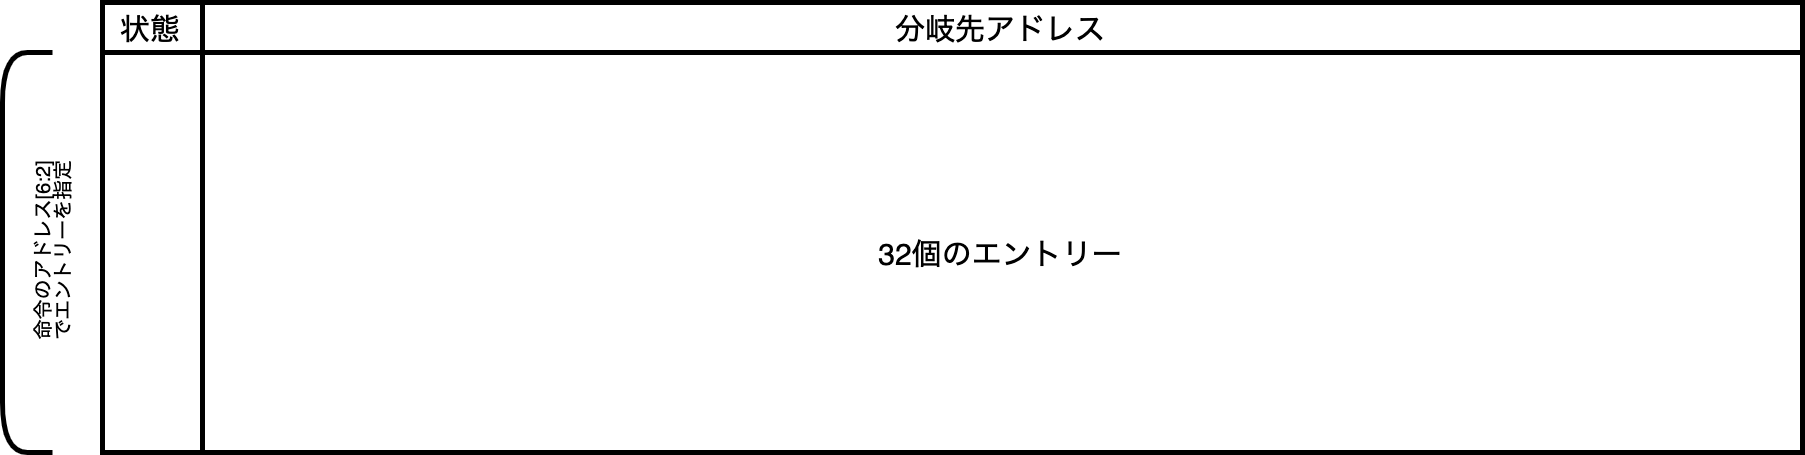
\includegraphics{../../images/predictor_table.png}
    }
    \caption{予測器の参照テーブル}
    \label{fig:predictor-table}
  \end{figure}

  \begin{table}[h!]
    \centering
    \begin{tabular}{|l|l|}
    \hline
    状態信号 & 分岐方向の予測 \\ \hline
    00 (STRONG\_NOT\_TAKE) & 分岐しない \\
    01 (WEAK\_NOT\_TAKE) & 分岐しない \\
    10 (WEAK\_TAKE) & 分岐する \\
    11 (STRONG\_TAKE) & 分岐する \\ \hline
    \end{tabular}
    \caption{予測器の状態信号と分岐方向の予測}
    \label{table:predictor-state}
  \end{table}

  命令メモリからフェッチした命令が予測の対象命令である時に, 
  参照テーブルのエントリーの状態信号と分岐先アドレスを元に, 
  分岐方向と分岐先アドレスを予測する.
  なお, 予測の対象命令ではない時に, 「分岐しない」と予測する.

  \subsubsection{予測期の参照テーブルの更新}
  分岐方向, または分岐先アドレスの結果が判明すると, 
  予測が成功したかどうかを元に, 予測器の参照テーブルの更新を行う.
  参照テーブルの該当エントリーに対し, 
  状態信号を図\ref{fig:predictor-state-transition} のように更新し, 
  分岐先アドレスを ALU で計算された分岐先アドレスに更新する.

  \begin{figure*}
    \centering
    \resizebox{1.5\columnwidth}{!}{
      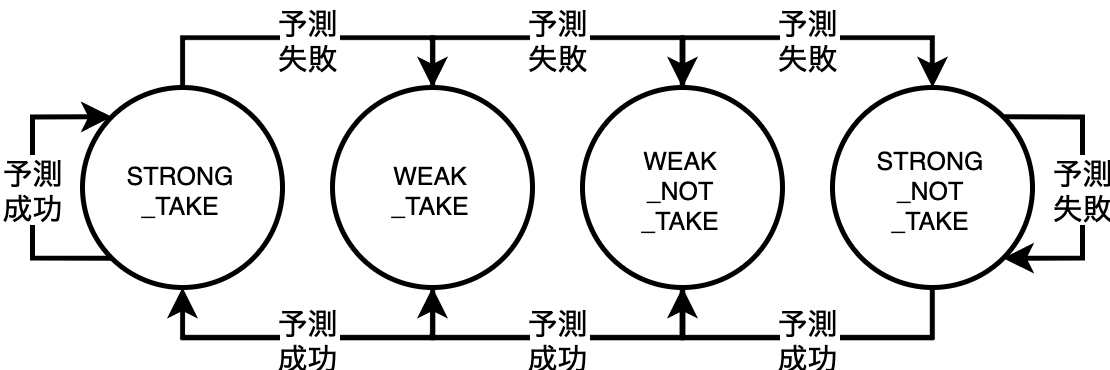
\includegraphics{../../images/predictor-state-transition.png}
    }
    \caption{$2\unit{\bit}$ 予測器: 状態遷移図}
    \label{fig:predictor-state-transition}
  \end{figure*}

  \subsubsection{分岐予測の評価と論理合成}
  エントリー数が 32個の参照テーブルをもつ分岐予測器を搭載したプロセッサを, 
  MiBench ベンチマークプログラムで実行クロックサイクル数とミス率を測定した後に, 論理合成を行った.
  実行クロックサイクル数の結果を表 \ref{table:mibench-improved} に, 
  ミス率の結果を表 \ref{table:miss-rate} に, 
  論理合成の結果を表 \ref{table:logic-synthesis-improved} に示す.

  \begin{table*}[bp]
    \centering
    \begin{tabular}{|c|r|r|}
      \hline
      ベンチマークプログラム & \multicolumn{1}{c|}{\begin{tabular}[c]{@{}c@{}}クロックサイクル数\\ (分岐予測実装前)\end{tabular}} & \multicolumn{1}{c|}{\begin{tabular}[c]{@{}c@{}}クロックサイクル数\\ (分岐予測実装後)\end{tabular}} \\ \hline
      stringsearch & 10594 & 6966 \\
      bitcnts & 56040 & 44680 \\
      dijkstra & 4079473 & 3048011 \\ \hline
    \end{tabular}
    \caption{分岐予測実装前後のプログラム実行クロックサイクル数}
    \label{table:mibench-improved}
  \end{table*}

  \begin{table*}[]
    \centering
    \begin{tabular}{|c|r|r|r|}
    \hline
    ベンチマークプログラム & \multicolumn{1}{c|}{分岐予測対象命令数} & \multicolumn{1}{c|}{予測失敗命令数} & \multicolumn{1}{c|}{予測失敗率 {[}\%{]}} \\ \hline
    stringsearch & 2113 & 131 & 6.20 \\
    bitcnts & 9930 & 690 & 6.95 \\
    dijkstra & 869932 & 12886 & 1.48 \\ \hline
    \end{tabular}
    \caption{分岐予測の予測失敗率}
    \label{table:miss-rate}
  \end{table*}

  % TODO
  % エントリ数を変化させて試したことを書いたなら、32より小さいテーブルサイズを選択しなかった理由を書いた方がいいね。
  % たぶん、論理合成が現実的な時間で済んで、かつ最もミス率が小さいからこれを選択したんだよね。
  参照テーブルのエントリー数を変化させて同じ項目で評価を行ったが, 
  32個以上の参照テーブルをもつ場合の論理合成にかかる時間が長かったため, 
  32個のエントリーを選んだ.

  % 伊織先輩:
  % ここの内容は全体的に検討が必要かな。
  % そもそもレジスタやメモリって容量にかかわらず初期化をするものだからね。
  %
  % \subsubsection{さらに改善できる点}
  % 今回の分岐予測の参照テーブルの実装方法であれば, 
  % シミュレーション上でしか, 正確な結果, または, 報告した通りの性能向上が出せない可能性がある.
  % シミュレーションの環境において, あるエントリーの状態信号が初期化されていない時, 
  % その信号は \verb|00|, \verb|01|, \verb|10|, \verb|11| のどれでもなく, \verb|xx| である.
  % ここで, Verilog-HDL で $2\unit{\bit}$ の条件文をもつ \verb|case| 分を使えば, 
  % \verb|default| で \verb|xx| の信号に対する処理ができる.
  % 今回の実装において, 状態信号が \verb|xx| の場合, 
  % 予測を \verb|WEAK_NOT_TAKEN| と出力するように記述している.
  % しかしながら, 実機では \verb|xx| の信号が存在しないため, 
  % この実装が実機上どんな動作をするかがわからない.
  % また, エントリー数が 32 個以上の参照テーブルを実装すれば, 
  % 参照テーブルがメモリとして論理合成される.
  % プロセッサのリセット時に全てのエントリーを 0 にリセットすることが現実的ではない.
  % そのため, 参照テーブルの実装方法を変えるか, 参照テーブルを使わない実装方法に変える必要がある.

\end{document}
